\chapter{Анализ литературы, патентов и обзор практики рецикла урана + Результаты исследований}\label{ch:ch1}

\section{Промышленный опыт}\label{sec:ch1/sec1}
Так как зарубежный опыт рецикла ядерного топлива исторически базируется на однократном использовании MOX-топлива, в данной работе будем опираться на Российский опыт возврата топлива в ЯТЦ \cite{international2003iaea}. К тому же, по части повторного использования урановой составляющей, отечественную ядерную индустрию можно считать глобальным лидером.  Эта практика вовлечения регенерата урана в топливные циклы энергетических реакторов базируется на смешении регенератов урана, извлекаемых из ОЯТ ВВЭР и ОЯТ транспортных реакторов с высоким содержанием U-235. Такая схема реализована для производства исходного сырья для изготовления топлива РБМК на заводе РТ-1 \cite{volkVozvratUranaIz2010}. Более того, этот вариант также апробирован для изготовления опытных ТВС для реакторов ВВЭР \cite{proselkovAnalizVozmozhnostiIspolzovaniya2003}, требующих более высокого уровня обогащения. 

дообогащение регенерата до необходимого для повторного использования в энергетических ядерных реакторах уровня концентрации изотопа 235U может быть проведено на имеющихся в нашей стране промышленных разделительных мощностях, основанных на центробежном методе разделения. 

\section{Потребности в соответствии с глобальной стратегией индустрии}\label{sec:ch1/sec2}


\subsection{Требования}\label{sec:ch1/sec1.1}
Согласно планам Росатома, для обеспечения конкурентоспособности на рынке зарубежных топливных поставок для легководных энергетических реакторов, следует предложить решение, обеспечивающее замыкание (пускай пока что и частичное) ЯТЦ. Подразумевая несовместимость опции MOX-топлива с ВВЭР (отсутствует лицензия) и с многократным рециклом, а также выигрышность варианта REMIX категории В, который связан с необходимостью обогащения урана, сконцентрируемся на подборе каскадной схемы для производства НОУ, способной обеспечить наилучшее решение, отвечающее следующим критериям. В обязательном порядке:

\begin{enumerate}
  \item Соответствие необходимым требованиям (спецификациям), предъявляемые к свежему топливу в целом. Может быть сформулировано как удовлетворение ограничений на присутствие нежелательных четных изотопов урана (возникших при облучении топлива и последующем хранении). Так, в соответствии с распространенным стандартом для низкообогощенного урана ASTM C996 - 15 \cite{c26committeeSpecificationUraniumHexafluoride}:
  \begin{enumerate}
    \item концентрация изотопа $^{232}$U в конечном продукте строго ограничена $5\cdot10^{-7}$\%, а иногда и $2\cdot10^{-7}$\%.
    \item Отношение изотопов $^{234}$U и $^{235}$U в продукте не должно превышать 0.02.
    \item $^{236}$U должен быть скомпенсирован дополнительным количеством делящегося $^{235}$U в продукте. В простейшем случае это количество составляет $^{236}$U$\cdot0.29$.
  \end{enumerate}
  \item Вовлечение максимально возможной доли делящегося изотопа U-235 в топливный цикл, что соответствует критерию экономии природного урана
\end{enumerate}

Может быть дополнено следующими условиями (пожеланиями):
\begin{enumerate}
  \item Вывод из топливного цикла балластных вредных четных изотопов посредством изотопного разделения, в ходе которого и происходит "повторное" обогащение регенерата. Концентрации нежелательных искусственных изотопов могут быть минимизированы до некоторой степени, когда это возможно, для многократной переработки, избегая их накопления, применяя разбавление изотопными композициями без искусственных изотопов, а также схемы очистки (см. далее).
  \item Использовать восстановленный уран на единицу продукта НОУ в необходимой пропорции (~ 0.93), что соответствует возврату в топливный цикл в виде 1 кг свежего топлива 1 кг ОЯТ.
  \item Предотвращение нежелательных потерь работы разделения в ходе операции разделения изотопов.
  \item Избежание накопления высокотоксичных отходов.
  \item Предел допустимой концентрации $^{235}$U на любом из стадий производства может быть ограничен лицензией обогатительного комбината. Так, например на СХК, такое ограничение составляет 5\%, что запрещает б`ольшую часть схем, предназначенных для дообогащения регенерата.
\end{enumerate}

В целом, политика вовлечения регенерированного урана в ЯТЦ позволяет в базовом варианте достигать экономии природного урана на уровне 11--20\% и многократного снижения объемов высокоактивных радиоактивных отходов за счет переработки ОЯТ \cite{delculAnalysisReuseUranium2009}. Возможность же осуществлять многократный рецикл урана и курс на удлинение (пролонгацию) топливных кампаний, связанный с повышением исходного уровня обогащения, открывает перспективы еще б`ольших преимуществ повторного использования делящегося материала.
Все это делает актуальным разработки каскадных обогатительных схем, направленные на решение задачи вовлечения урановой составляющей отработанного топлива в топливный цикл легководных энергетических реакторов.


\subsection{Источники ограничений использования регенерата}\label{sec:ch1/sec1.2}
Наличие перечисленных строгих ограничений пункта 1 связано с нейтронно-физическими и радиационными свойствами четных изотопов из ряда $^{232,234,236}$U \cite{smirnovEvolutionIsotopicComposition2012, proselkovAnalizVozmozhnostiIspolzovaniya2003, dudnikovInfluence236UEfficacy2016}. Так, первый в этом ряду изотоп $^{232}$U является особенно опасным источником радиационного загрязнения из-за интенсивного гамма-излучения (2.6 МэВ), испускаемого дочерним короткоживущим $^{208}$Tl (3.65 мин.) \cite{article}. 
$^{232}$U вместе $^{234}$U превносят альфа-частицы в смесь гексафторида урана ($UF_6$ -- соединение, используемое в процессе обогащения урана \cite{orlovWayObtainUranium2015, orlovDesublimationPurificationTransporting2017}), вероятно, приводя к его диссоциации \cite{kryuchkovObogashchennyyUranDobavleniem2007, bernhardtRadiationEffectsAlpha1958}. $^{236}$U действует как паразитный поглотитель нейтронов, который препятствует цепной реакции. Этот эффект отравления реактора должен быть скомпенсирован в простейшем случае дополнительным количеством делящегося $^{235}$U в продукте. Записывая уравнение, для обеспечения требуемого эквивалента уровня обогащения по $^{235}$U, к заданной концентрации для случая обогащения природного урана необходимо обеспечить добавку, определяемую наличием $^{236}$U -- паразитного нейтронного поглотителя:
$C_{235 e q}^{P}=C_{235 n a t}^{P}+K_{236} \times C_{236}^{P}$,
где $K_{236}$ -- коэффициентом компенсации реактивности, значение которого может лежать в пределах 0.2--0.6 \cite{delagarzaMulticomponentIsotopeSeparation1961, delculAnalysisReuseUranium2009}.

Как альтернатива, может рассматриваться уравнение $C_{235 e q}^{P}=f\left(C_{236}^{P}\right)$, вид которого будет определяться аппроксимацией, соответствующей сбалансированной ядерной реакции, полученной в ходе нейтронного-физического расчета для заданной реакторной кампании.
Стоит отметить, что изотоп $^{234}$U имеет тенденцию захватывать нейтрон и превращаться в делящийся $^{235}$U, что должно уменьшить необходимую компенсацию $^{236}$U \cite{dyachenkoIspolzovanieRegenerirovannogoUrana2012}, хотя это обычно не учитывается ввиду порядка малости.

\section{Сравнительный анализ известных схем}\label{sec:ch1/sec2}

Ниже представлен анализ современных подходов к проблеме повторного обогащения регенерата, основанных на технологии газовой центрифуги (ГЦ) и достижениях каскадной теории разделения многокомпонентных смесей. Так как технология ГЦ на сегодня является лидирующей в промышленном производстве обогащенного урана, кратно превосходя своего ближайшего конкурента -- газовую диффузию в рентабельности и энергоэффективности, ограничимся ею в своем рассмотрении \cite{rothwellCostStructureInternational2008}.
Оставляя также в стороне вопросы, связанные с химической переработкой для получения восстановленной урановой изотопной смеси, предлагается рассмотрение усовершенствованных конфигураций каскадов газовой центрифуги для повторного обогащения этой смеси. При этом, как и условились ранее, ограничимся регенерированным ураном, полученным из ОЯТ коммерческого легководного реактора -- российского ВВЭР.

\subsection{Основы теории разделения в каскадах}\label{sec:ch1/sec2.1}

\textcolor{red}{Базовые понятия (разделительный элемент, симметричн.-противоточное соединений, каскад) + основные уравнения (балансы, срез, коэффициенты разделения ступеней)}

Обогащение переработанного урана является задачей разделения изотопов многокомпонентной изотопной смеси, тогда как обогащение природного урана представляет собой более простую задачу разделения бинарной смеси. Сложность работы с многокомпонентным изотопным составом регенерата заключается в необходимости разработки теории исключительно для разделения многокомпонентных изотопных смесей (хотя это касается и разделения стабильных изотопов некоторых химических элементов, например вольфрама).

Область моделирования разделительных каскадов на сегодня владеет обширным набором расчетных моделей, которые могут быть применены к задаче по обогащению регенерата. В нашем случае для разделения смеси регенерата может быть применен ряд специальных теоретических моделей. Наиболее общая модель здесь называется «квазиидеальным» каскадом, где предполагается постоянство срезов ступеней ($\theta$ делит входной поток на $\theta$ и $1 - \theta$ соответственно) по каскадным ступеням \cite{yamamotoMulticomponentIsotopeSeparating1978}. В настоящее время он используется в двух приближениях: с низким (слабым) обогащением (Q-каскад \cite{borisevichNewApproachOptimize2011, kolokoltsovDesignCascadesSeparating1970, zengQCascadeExplanation2012}) и неограниченным (произвольным) обогащением (квазиидеальный каскад \cite{sulaberidzeSpecialFeaturesEnrichment2006}). Обе математические модели предлагают выбор профиля потока в каскаде, следовательно, дают возможность добиться наиболее эффективного обогащения целевого компонента. Такой подход значительно упрощает как анализ закономерностей массообмена в каскаде для многокомпонентного разделения, так и соответствующий расчет. В исследованиях, как правило, когда обогащенный переработанный уран обогащается многопоточными схемами, часто используется модель R-каскада (Matched Abundance Ratio Cascade-MARC \cite{delagarzaMulticomponentIsotopeSeparation1961, woodEffectsSeparationProcesses2008, kazukihidaSimultaneousEvaluationEffects}). Это особый случай `квазиидеального' каскада. Здесь условие отсутствия смешивания выполняется для выбранной пары компонентов (например, это могут быть изотопы $^{235}$U и $^{238}$U). Еще раз подчеркнем, что все вышеупомянутые каскадные модели действуют как физически эквивалентные представления. 

Стоит упомянуть, что существует альтернативный подход к каскадному расчету, когда набор из шести уравнений включает 10 основных внутренних параметров:

$L_{i}, C_{i}, L_{i}^{\prime}, C_{i}^{\prime}, L_{i}^{\prime \prime}, C_{i}^{\prime \prime}, q_{i}, \theta_{i}, N_{i}, l_{i}$,

где $L_{i}, L_{i}^{\prime}, L_{i}^{\prime \prime}$ и $C_{i}, C_{i}^{\prime}, C_{i}^{\prime \prime}$ -- 
это потоки питания, продукта и отвала и их концентрации соответственно; $q_{i}$ -- коэффициент разделения; $\theta$ -- коэффициент деления потока на ступени (срез); $N_{i}$ -- число ступеней; и $l_{i}$ -- поток питания отдельной центрифуги.

Эти параметры связаны шестью уравнениями:
$\begin{array}{c}
  {L_{i}^{\prime}+L_{i}^{\prime \prime}=L_{i}} \\
  {L_{i}^{\prime} C_{i}^{\prime}+L_{i}^{\prime \prime} C_{i}^{\prime \prime}=L_{i} C_{i}} \\
  {q_{i}=\frac{(1-C_{i}^{\prime \prime}) C_{i}^{\prime}}{(1-C_{i}^{\prime}) C_{i}^{\prime \prime}}} \\
  {q_{i}=q_{i}\left(l_{i}, \theta_{i}\right)} \\
  {\theta_{i}=\frac{L_{i}^{\prime}}{L_{i}}} \\
  {l_{i}=\frac{L_{i}}{N_{i}}}
\end{array}$


Помимо этих 6$n$ соотношений, описывающих отдельные ступени, необходимо учитывать уравнение, связывающее межкаскадные потоки -- балансные уравнения, вид которых зависит от рассматриваемой схемы коммутации ступеней. Для каскада, показанного на рис. 1, эти уравнения записаны в виде:

$\begin{array}{c}
  {L_{1}=L_{2}^{\prime \prime}, \ldots ; L_{i}=L_{i-2}^{\prime}+L_{i+1}^{\prime \prime}, \ldots ;} \\
  {L_{1} C_{1}=L_{2}^{\prime \prime} C_{2}^{\prime \prime}, \ldots ; L_{i} C_{i}=L_{i-2}^{\prime} C_{i-2}^{\prime}+L_{i+1}^{\prime \prime} C_{i+1}^{\prime \prime}, \ldots}
\end{array}$

В дополнение к этим соотношениям необходимо учитывать граничные условия, относящиеся к внешним и внутренним параметрам. Например для симметричного противоточного каскада, они выражаются соотношениями: 
$P=L_{n}^{\prime} ; C_{P}=C_{n}^{\prime} ; W=L_{1}^{\prime \prime} ; C_{W}=C_{1}^{\prime \prime}$

, которые выполняются для каждой ступени каскада \cite{palkinDeterminationOptimalParameters2012}. Эти уравнения описывают отношения между соседними ступенями и, опираясь на ряд граничных условий, могут служить эффективной репрезентацией каскада.

\subsection{Основные модификации стандартного (ординарного) каскада, используемого для обогащения природного урана}\label{sec:ch1/sec2.2}
Далее представлен анализ современных подходов к проблеме повторного обогащения регенерата и соответствующий набор методов, основанных на технологии газовой центрифуги и достижениях теории каскадов. Эти методы соответствуют набору каскадных схем, предложенных для решения задачи возврата регенерированного урана в топливный цикл энергетических реакторов.
Начнем со схемы, основанной на базовом (ординарном/трехпоточном) каскаде.
Его можно применять, например, следующими способами (рис. \ref{fig:diagram1}) \cite{smirnovKaskadnyeShemyZadachah2012}:
\begin{enumerate}
  \item Совместное обогащение смесей природного и регенерированного урана.
  \item Производство обогащенной фракции из регенерата и последующее ее разбавление природной урановой смесью.
  \item Предварительное обогащение природного урана немного больше, чем необходимо для получения НОУ требуемого качества, с последующим разбавлением его регенератом.
\end{enumerate}

\begin{figure}[ht]
  \centerfloat{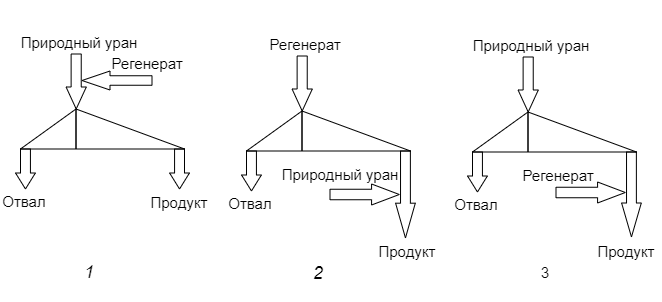
\includegraphics[scale=0.7]{cascades/diagram1}}
  \caption{Двойной каскад}\label{fig:diagram1}
\end{figure}

\textcolor{red}{Или нагляднее в работе для NET?}

Соотношение между расходом регенерата и разбавителем природного происхождения определяется пределом содержания $^{232}$U в конечном продукте и компенсацией отрицательной реактивности $^{236}$U. В то же время концентрация $^{235}$U там не должна быть ниже, чем требуется для НОУ с определенными свойствами.

Основным преимуществом таких схем является простота реализации, поскольку нет необходимости в нестандартной модификации каскада. При этом, как недостаток можно выделить потери работы разделения, возникающие из-за смешения потоков с различными изотопными концентрациями $^{235}$U. 
Однако недостаточность такой простейшей модификации для решения задачи вовлечения регенерата в условия многократного рецикла будет показана в \ref{sec:ch1/sec3.1}.


\subsection{Усовершенствованные конфигурации каскадов, например, с несколькими дополнительными внешними потоками (многопоточные схемы)}\label{sec:ch1/sec2.3}
Чтобы превратить базовый каскад в многопоточный, мы должны применить дополнительные питания или исходящие потоки побочных продуктов. Так, дополнительные входные потоки сырья действуют как разбавители, а при дополнительном удалении образуется очищенный промежуточный продукт.

\subsubsection{Применение дополнительных обособленных потоков питания}
Чтобы преодолеть недостатки, связанные с разделительными потерями упомянутых схем (рис. \ref{fig:diagram1}), трехпоточный каскад был модернизирован до многопоточного каскада с дополнительным потоком \cite{smirnovKaskadnyeShemyZadachah2012}. Здесь регенерат `направляется' (сублимируется с помощью конденсационно-испарительной установки из твердой в газообразную форму \cite{orlovDesublimationPurificationTransporting2017}) в каскад через отдельную точку подачи -- на ступень, отличную от ступени подпитки природной смесью (рис. !!!). Этот прием позволяет избежать неблагоприятных последствий смешения потоков с различными концентрациями $^{235}$U, располагая дополнительный входной поток там, где концентрации внешнего и внутреннего потоков в $^{235}$U совпадают (внешние потоки являются источником питания каскада; внутренние потоки -- потоки, циркулирующие внутри каскада). Поэтому очевидное практическое преимущество такого метода, по сравнению с предыдущими обычными схемами, связано с отсутствием потерь работы разделения \cite{smirnovKaskadnyeShemyZadachah2012, sulaberidzeQuasiidealCascadesAdditional2006}.

Использование большого количества природного урана для разбавления регенерата является обычным недостатком вышеупомянутых каскадных схем (рис. \ref{fig:diagram1} +!!!), поскольку необходимо, прежде всего, снизить содержание $^{232}$U в продукте. Тем не менее, при повторном использования топлива ВВЭР, такой подход может обеспечить значительную экономию природного урана $\approx$16\% только лишь на первом рецикле (а ведь это возможно осуществлять многократно, увеличивая экономию природного ресурса), как показано в оценках в \cite{smirnovEvolutionIsotopicComposition2012}. Но `полный' возврат ОЯТ в топливный цикл (использование 1 кг ОЯТ на 1 кг НОУ продукта) достижим в этом случае только для изотопных составов первого (иногда второго) рецикла, что означает невозможность с помощью такой схемы обеспечить требуемую пропорцию вовлечения регенерированного урана в условиях многократного рецикла \cite{smirnovApplyingEnrichmentCapacities2018}.
Для рассматриваемого каскада с двумя питаниями, начиная с третьего цикла, требуемый уровень использования регенерата становится невозможным из-за ухудшения изотопного состава урана и наличия ограничений на изотопы $^{232,236}$U.
Так, в \cite{smirnovApplyingEnrichmentCapacities2018} были рассчитаны экономия природного урана и работы разделения (РР) и показано, что для каждого цикла можно достичь примерно 20\% экономии природного урана до того, как к третьему циклу повторного использования происходит значительная деградация изотопного состава.
Чтобы повысить пределы экономии природного урана, оставаясь в рекомендованных пределах, мы должны искать альтернативный разбавитель. Например, это может быть обедненный уран (так называемые «хвосты» (или отвалы) -- побочный продукт процесса обогащения). Это может быть плодотворно использовано для частичной замены природного урана в качестве основного разбавителя, хотя этот материал часто рассматривается как «отходы». Такая конфигурация изображена на рис. !!!!. , описание же математической модели приведено в \cite{smirnovEnrichmentRegeneratedUranium2014} .
\textcolor{red}{Или можно как у Маслюкова запрудить мат.моделями?}
Основным преимуществом его использования является возможность существенной экономии природного урана, демонстрируя устойчивую экономию половины природного урана
Эта особенность делает эту схему многообещающей, поскольку она сочетает соотношение двух разбавителей для достижения надлежащей экономии природного урана или разделительной работы, что позволяет «настраивать» каскад для конкретных изотопных составов смесей и для текущих цен. Кроме того, такой вариант полезен для решения проблемы накопленных количеств обедненного урана [43]. Поскольку UF6 является довольно агрессивным веществом, его хранение связано с определенными затратами, и емкости для хранения следует время от времени заменять из-за коррозионных процессов [44,45].
Такая схема (рис. 5), как и предыдущая, могла бы обеспечить полный возврат урана в ядерный топливный цикл для двух начальных циклов, но это невозможно для серии последовательных циклов из-за быстрого накопления малых изотопов и невозможность как-то очистить композиции от этих нежелательных компонентов в таких схемах [42]. Это ограничение было ясно видно в первых двух таблицах работы [42], показывающих эволюцию изотопного состава при многократной переработке.

Тут то и возникает проблема очистки изотопных составов. Итак, давайте опишем способы, как мы могли бы удалить нежелательные изотопы из системы, каким-то образом очистив смесь. Это может быть сделано со схемами, которые позволяют извлекать промежуточный продукт, или с мульти-структурами (несколько последовательных каскадов, например, двойная обычная каскадная схема), которые будут описаны далее.


Однако во всех рассмотренных схемах заметное снижение содержания изотопов $^{232,234,236}$U в финальном НОУ достигается, прежде всего, за счет разбавления регенерата внутри каскада смесями, имеющими происхождение от природного урана (НОУ, ОГФУ, или сам природный уран). Далее будет показано, что приведенная классификация является условной, и будет предложена дихотомия, выделяющая схемы-разбавители и схемы-очистители (от четных изотопов). Итак, давайте опишем способы, как мы могли бы удалить нежелательные изотопы из системы, каким-то образом очистив смесь. Это может быть сделано со схемами, которые позволяют извлекать промежуточный продукт, или с составными схемами (несколько последовательных каскадов, например, двойной каскад). Остановимся на первых поподробнее.

\subsubsection{Применение дополнительных потоков отбора}

Схемы, называемые каскадами с промежуточным продуктом предназначены для «очистки» (по существу, при разбавлении природным ураном) от второстепенных изотопов представлена ниже (рис. ___) [21,30]. Здесь в качестве продукта получают НОУ, а в качестве промежуточного продукта получают композицию с пониженным содержанием второстепенных изотопов.


\subsection{Комбинации нескольких каскадов (составные схемы)}\label{sec:ch1/sec2.4}
Под составными схемами будем подразумевать коммутации единичных каскадов в единую составную структуру.

Приведенный критический анализ различных каскадных схем позволяет нам ближе рассмотреть возможные области применения и, таким образом, позволяет более осознанно выбирать конфигурацию для каждой обособленной практической задачи. То есть не представляется возможным остановиться на единственном универсально оптимальном варианте, а лишь можно отметить частные положительные стороны. Таким образом, этот обзор может быть использован в качестве основы для дальнейших научных, технических и технико-экономических обоснований крупномасштабного повторного использования ядерных материалов в различных топливных циклах. Такое исследование и будет проведено далее в данной диссертационной работе.


\section{Расчетные исследования известных схем}\label{sec:ch1/sec2}

\subsection{Обоснование ограничений использования ординарных схем (на основе ординарных каскадов)}\label{sec:ch1/sec3.1}
\textcolor{red}{Работа для NET, переписанная слово в слово}

Таким образом, анализ схем на основе базового трехпоточного каскада демонстрирует потребность в модификации компоновок разделительного оборудования в контексте многократного рецикла урана.

Подводя итог подраздела, известные на сегодняшний день  технические решения (подробно описаны в последующих разделах и Отчете о патентных исследованиях) основаны на:
-	разбавлении регенерированного урана материалами, не содержащими минорных компонентов (например, природным ураном), на входе в разделительный каскад, на выходе из разделительного каскада или внутри каскада при наличии в нем двух питающих потоков (регенерат и разбавитель);
-	получении регенерата с пониженным содержанием минорных изотопов в каскаде с двумя питаниями и двумя потоками продукта (отбора);
-	выделении из смесей регенерированного урана изотопа U-232 при помощи газа-носителя в последовательном соединении двух разделительных каскадов.

\subsection{Обоснование необходимости составных схем/схем с дополнительными потоками}\label{sec:ch1/sec3.1}
Отсюда и вытекает необходимость использовать составные каскадные схемы ввиду необходимости  `пространственного' разделения. Так двойная схема позволяет отделить минорные легкие изотопы $^{232}$U, $^{234}$U в независимом потоке отборной части каскада. Так, например, схема \ref{fig:double} позволяет во втором каскаде разделить потоки, выделив $^{235}$U в тяжелой фракции, направив $^{232}$U и $^{234}$U в легкую.

\begin{figure}[ht]
  \centerfloat{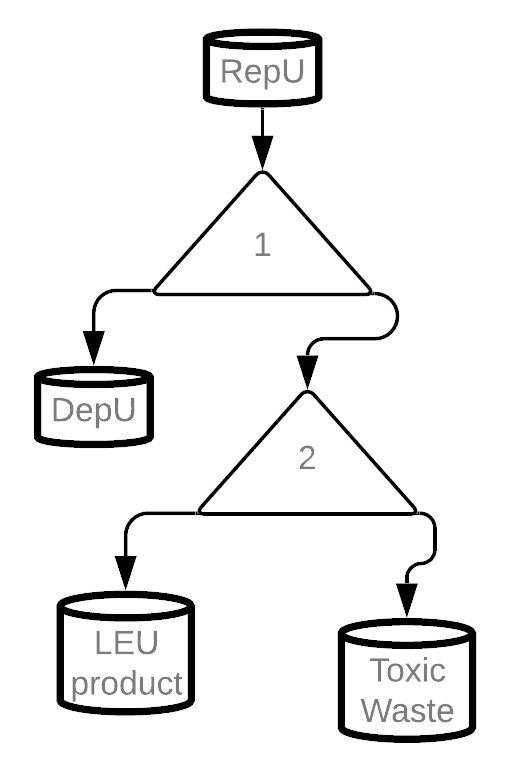
\includegraphics[scale=0.3]{cascades/double}}
  \caption{Двойной каскад}\label{fig:double}
\end{figure}

С появлением свойств такого рода у каскадов, вместо привычной дихотомии, выделяющей схемы с приставкой `много-' (многопоточные схемы, многокаскадные конфигурации), предлагается классифицировать каскады, используемые для обогащения регенерата, как разбавляющие или очищающие. Так, схема двойного каскада является очищающей, в отличие от схем, основанных на ординарном каскаде, работающих на принципе разбавления.  Хоть и любая таксономия арбитрарна, условная граница `касад-разбавитель' -- `каскад-балластоочиститель' гораздо лучше подчеркивает сущностные характеристики анализируемых схем, предназначенных для повторного обогащения урана.

\section{Разработка схем полного возврата}\label{sec:ch1/sec4}
В качестве модификации двойного каскада была предложена альтернативная каскадная схема, которая позволяет обеспечить возврат регенерата в цикл в соотношении 1:1. В этой схеме, изображенной 
на рисунке \ref{fig:vestnik}, первая часть (каскад 1) увеличивает 
концентрацию $^{235}$U со всеми более легкими изотопами ($^{232}$U и $^{234}$U) и направляет их (через выходящий поток в правой части на рисунке) ко второму каскаду, который будет концентрировать эти четные миноры в потоке загрязненного продукта \cite{smirnovObogashchenieRegenerirovannogoUrana2018}.
Хотя на этот раз приготовленная композиция разбавляется НОУ для контроля концентраций $^{232}$U и $^{234}$U в допустимых пределах и для управления соотношением рециклируемых материалов (для поддержания соотношения регенерата в питании каскада к нарабатываемому продукту на уровне 1:1, что формально соответствует полному возврату выгоревшего топлива в ядерный топливный цикл).

\begin{figure}[ht]
  \centerfloat{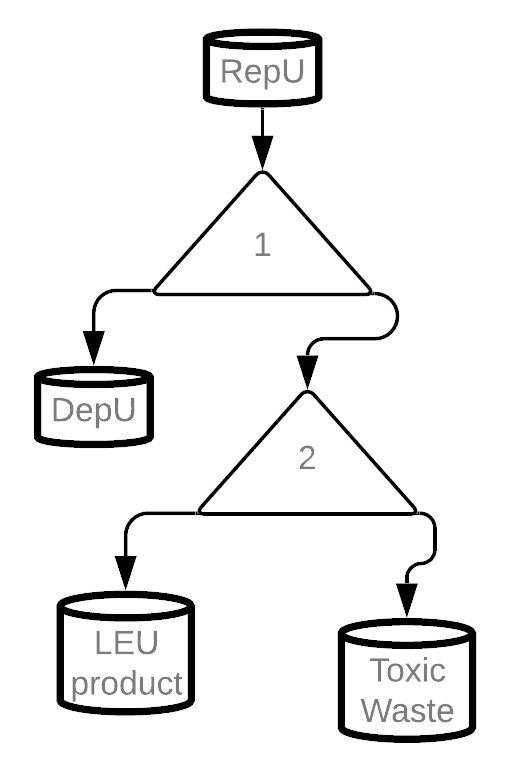
\includegraphics[scale=0.3]{cascades/double}}
  \caption{Двойной каскад с добавлением НОУ (тройной каскад)}\label{fig:vestnik}
\end{figure}

Хотя этот вариант и кажется идеальным, цена хранения побочного продукта из загрязненной смеси слишком высока, что мгновенно делает схему нежизнеспособной, если нет способов избежать такого негативного побочного эффекта.
Однако затем было предложено применить дополнительный каскад для производства НОУ из загрязненной смеси, сильно разбавленной обедненным ураном (которые имеют высокую концентрацию $^{235}$U около $\approx$20\%), чтобы получить конечный продукт в двух исходящих потоках и достичь значительной экономии природного урана ($\approx$38\%) даже для `грязной' композиции, которая уже была пятикратно рециклирована (рисунок \ref{fig:Tomsk}). Расчеты показали, что такой подход позволяет производить НОУ коммерческого качества, расходуя определенное количество переработанного урана и отвечая стандартным спецификациям для  $^{232}$U (и условиям, установленным для других четных изотопов). В то же время, предлагаемая схема обеспечивает большую экономию природного урана, чем большинство схем обогащения переработанного урана. Это могло бы также обеспечить широкомасштабную «мобилизацию» обедненного урана.

\begin{figure}[ht]
  \centerfloat{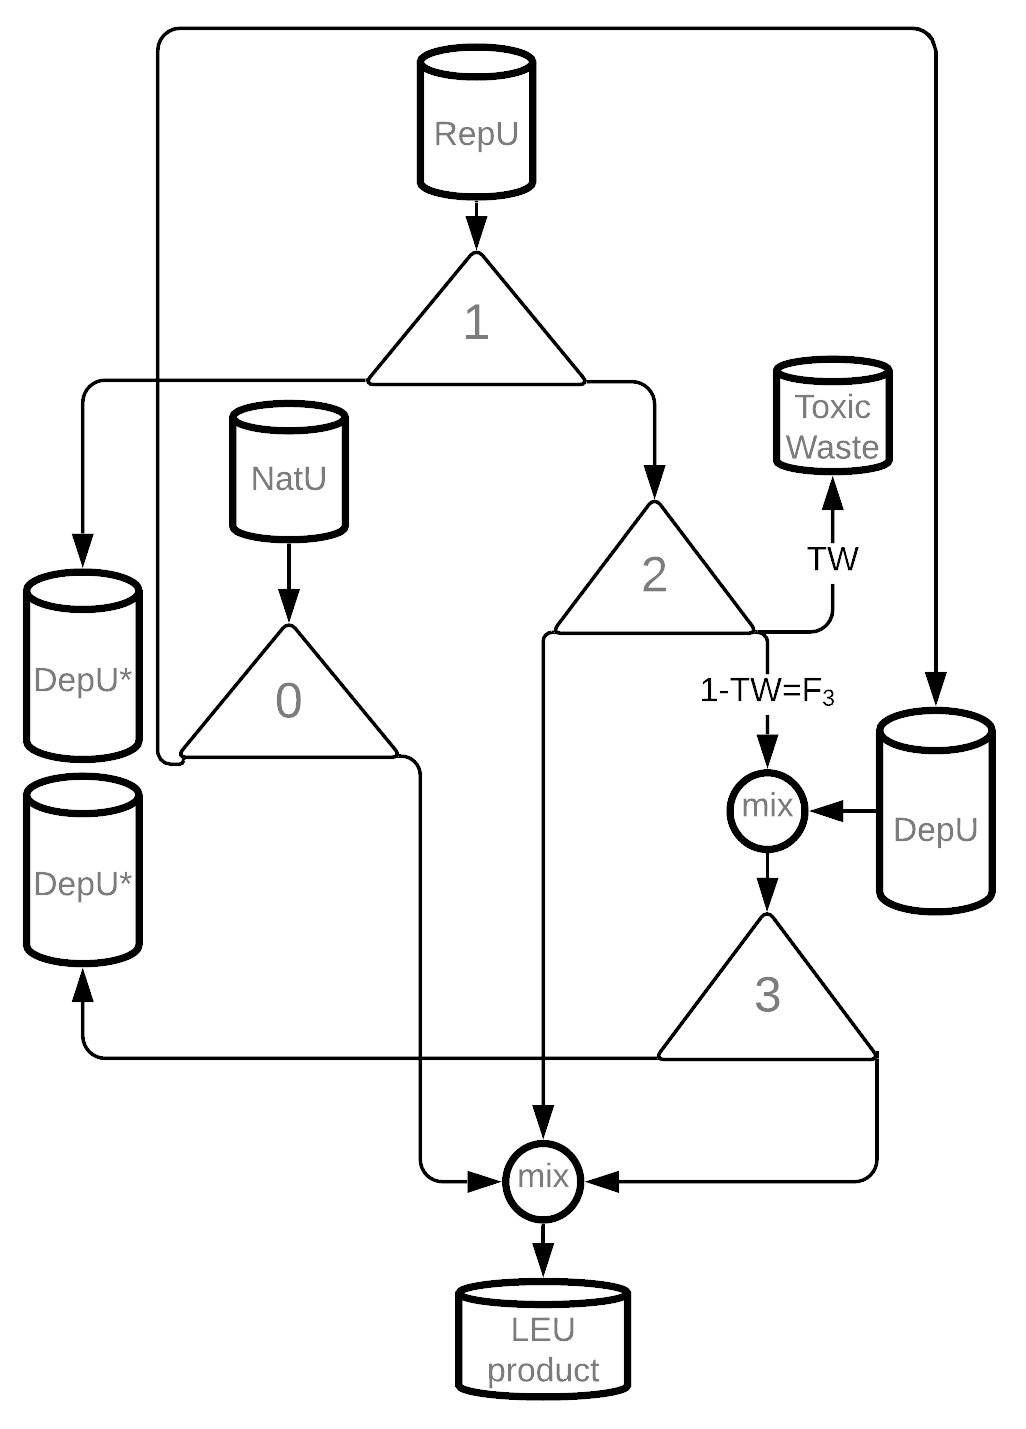
\includegraphics[scale=0.3]{cascades/Triple_Tomsk}}
  \caption{Тройной каскад с подмешиванием ОГФУ и НОУ-разбавителем}\label{fig:Tomsk}
\end{figure}

Затем, в качестве альтернативы была предложена схема рисунка \ref{fig:patent}), в которой на каскад с индексом 3 подается смесь грязного потока легкой фракции каскада 2, которая разбавляется обедненным гексафторидом урана до содержания $^{235}$U на уровне природного урана. Этот поток в дальнейшем разбавляется чистым природным ураном, пропорция которого подбирается для выполнения всех заданных условий.
\begin{figure}[ht]
  \centerfloat{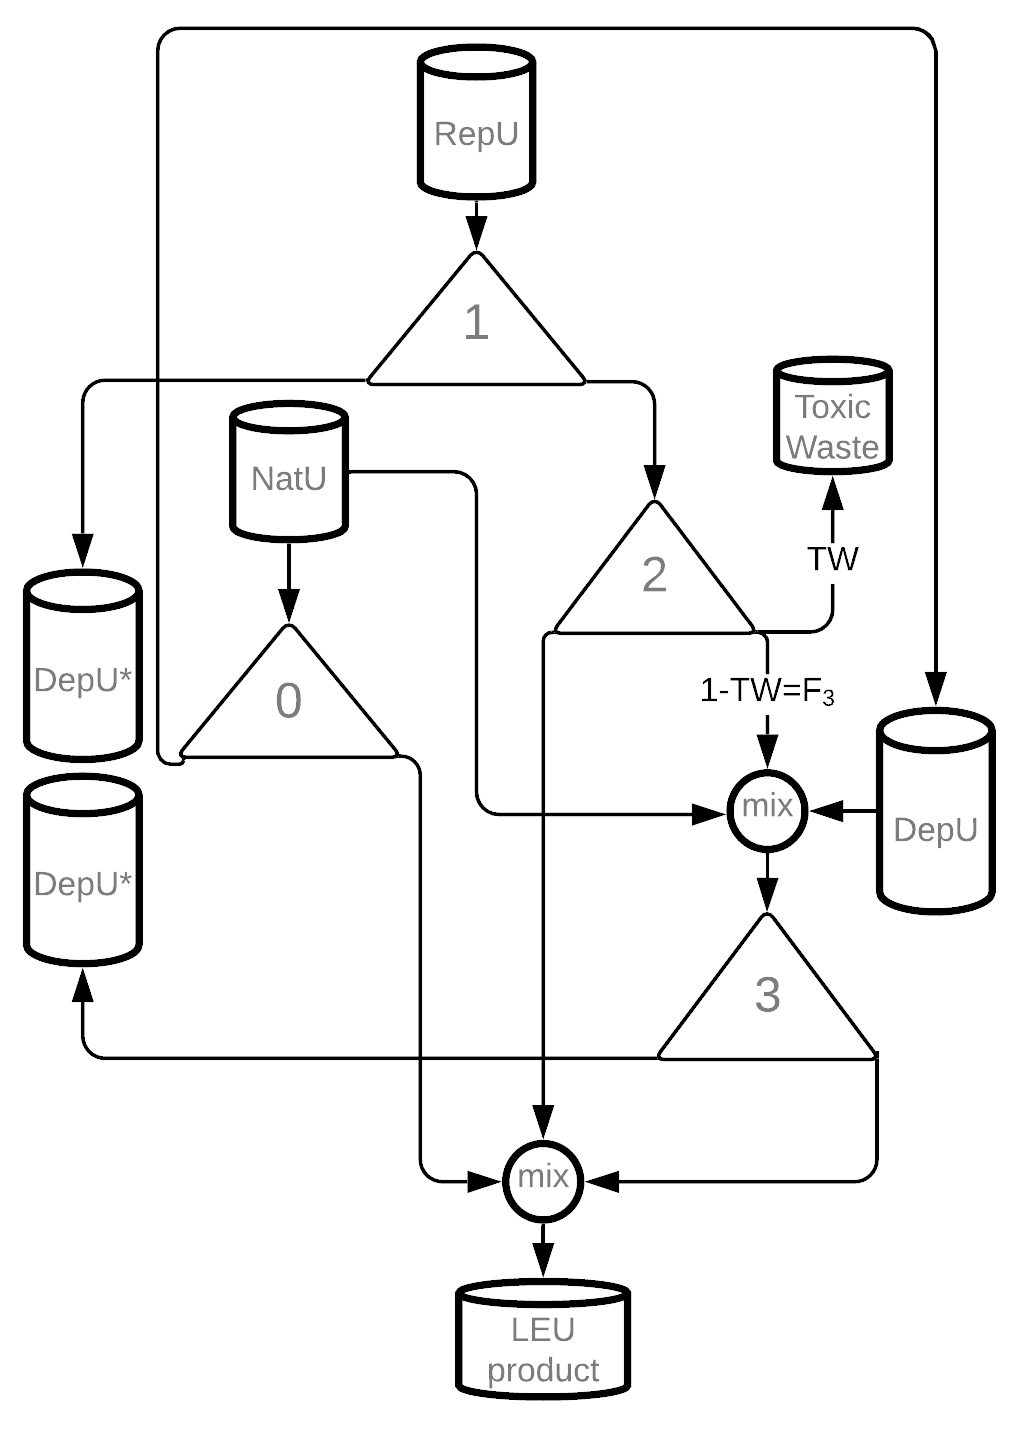
\includegraphics[scale=0.3]{cascades/triple_cascade_complete_return}}
  \caption{Тройной каскад с подмешиванием НОУ, ОГФУ и природного урана}\label{fig:patent}
\end{figure}

Как мы видим, такие схемы также очень ценны как инструмент для переработки всего количества выделенного урана.


\section{Прочие аспекты}\label{sec:ch1/sec5}

Использование регенерированного урана, помимо возможностей расширения ресурсной базы и сокращение отходов, необходимо рассмотреть и с иных позиций. Так, переработка ОЯТ для последующего использования зачастую рассматривается как нежелательная опция с позиций нераспространения ядерного оружия (позиция США в рамках GNEP), а технология газовой центрифуги и материал класса НОУ на сегодня рассматриваются экспертами как наиболее чувствительные \cite{nevinicaPovyshenieZashchishchennostiEksportnyh}. То есть, расширение применения двух ключевых технологии для возврата урана в цикл - гидрометаллургического восстановления и газоцентрифужного каскадного обогащения представляется, на первый взгляд, негативным с точки зрения вопроса сдерживания распространения ядерного оружия. Однако, если производство ядерного топлива ограничивается странами - глобальными лидерами в ЯЭ (как, к примеру, в рамках российской инициативы по созданию системы международных центров по предоставлению услуг ядерного топливного цикла), а неядерным державам, поставляется топливо на основе регенерата урана, ситуация в корне меняется. Благодаря нейтроно-физическим свойствам такого топлива, вариант его переключения представляется гораздо менее осуществимым. Это обусловлено как неизбежным высоким радиационным воздействием в случае операции переключения ядерного материала, сопровождающейся необходимостью его конверсии (несколько стадий) и обогащения, так и легкостью детектирования изъятия даже малых количеств делящегося материала. Помимо резкого снижения привлекательности материала на основе регенерата для создания ядерного уранового заряда, присутствие в нем U-236 значительным образом повышает выходную концентрацию Pu-238 в изотопном векторе плутония, уменьшая возможность его немирного переключения. Так, в работе \cite{solovevAnalizYadernogoToplivnogo2019} показано, что рециклирование РЕМИКС-топлива, приводит к накоплению четных изотопов в плутониевой фракции, повышая защищенность от несанкционированного переключения.


\subsection{Ядерное нераспространение. Анализ сценариев переключения}\label{sec:ch1/sec5.1}

\textcolor{red}{Последняя статья в АЭ по нераспространению:}

Рассмотрен модельный сценарий переключения ядерного материала из топлива легководного реактора типа ВВЭР-1000 или ВВЭР-1200,  изготовленного из регенерированного урана. Предполагали, что АЭС находится под гарантиями МАГАТЭ. Технической целью гарантий является предотвращение или своевременное обнаружение переключения значимого количества ядерных материалов (требования своевременности обнаружения переключения значимого количества ЯМ зависят от  его категории) \cite{ermakovVozmozhnyeProceduryGarantiy1987}. Так, в соответствие с \cite{ermakovVozmozhnyeProceduryGarantiy1987}, технической целью гарантий МАГАТЭ применительно к реактору ВВЭР-1000 является обнаружение переключения в течение года такого количества низкообогащенного урана, которое содержит более 75 кг $^{235}$U.
...с помощью:  надкритических центрифуг TC-12 компании URENCO \cite{borisevichIdealOptimumCascades2014}. 


Представленные зависимости наглядно демонстрируют, что период между инспекциями является временем, вполне достаточным для переключения. За рамками работы мы оставили вопрос химической конверсии (превращения оксидов U в фториды U и наоборот (и в металл)) \cite{orlovDesublimationPurificationTransporting2017}, однако это одна из необходимых технологий, требуемых для обогащения урана. 



